\section{}
\[
H(s)=\frac{10\,(1 - s)}{s+10}\,.
\]
\subsection{Bode-Diagramm}
\begin{center}
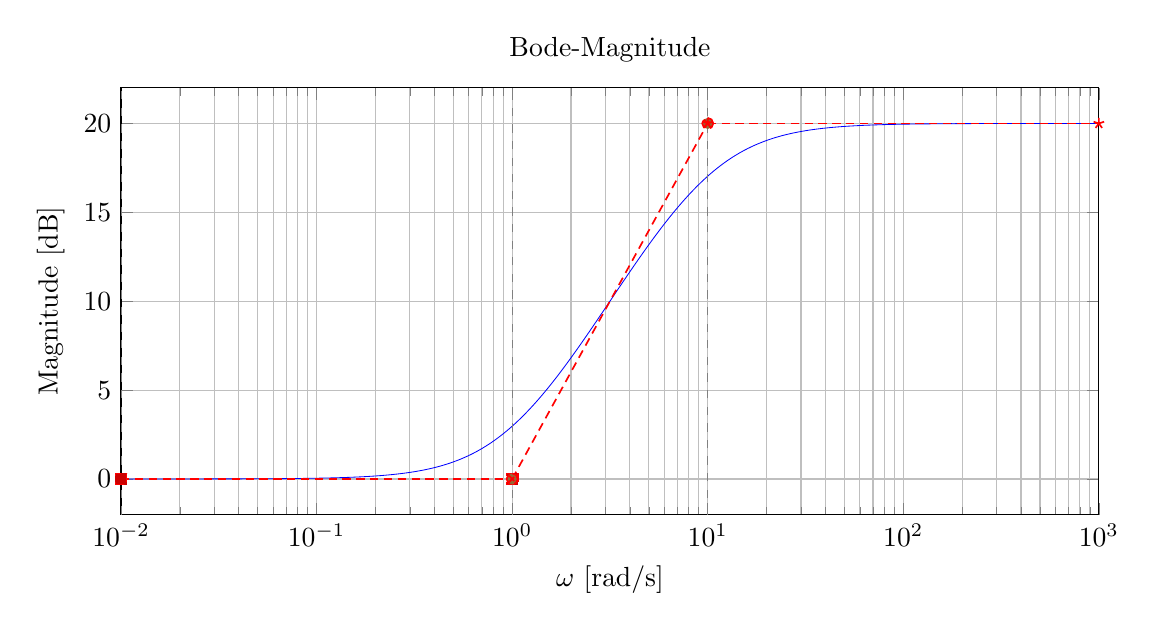
\begin{tikzpicture}
\begin{semilogxaxis}[
  width=14cm,height=7cm,
  xmin=1e-2,xmax=1e3,
  xlabel={$\omega$ [rad/s]},
  ylabel={Magnitude [dB]},
  grid=both,
  title={Bode-Magnitude}
]
\addplot[
  domain=1e-2:1e3,
  samples=600,
  mark=none,
  ytick distance=10,
  line width=0.3pt,
  blue
] {20 + 20*ln(sqrt(1 + x^2))/ln(10) - 20*ln(sqrt(100 + x^2))/ln(10)};
\addplot+[domain=1e-2:1,samples=2,dashed,dash pattern=on 3pt off 2pt,line width=0.6pt,red] {0};
\addplot+[domain=1:1e1,samples=2,dashed,dash pattern=on 3pt off 2pt,line width=0.6pt,red] {20*ln(x)/ln(10)};
\addplot+[domain=1e1:1e3,samples=2,dashed,dash pattern=on 3pt off 2pt,line width=0.6pt,red] {20};
\draw[gray,dashed] (rel axis cs:0,0) -- (rel axis cs:0,1);
\draw[gray,dashed] (axis cs:1,\pgfkeysvalueof{/pgfplots/ymin}) -- (axis cs:1,\pgfkeysvalueof{/pgfplots/ymax});
\draw[gray,dashed] (axis cs:10,\pgfkeysvalueof{/pgfplots/ymin}) -- (axis cs:10,\pgfkeysvalueof{/pgfplots/ymax});
\node[gray,anchor=south east] at (axis cs:1,\pgfkeysvalueof{/pgfplots/ymax}) {\scriptsize Nullstelle $\omega_z=1$ (RHP)};
\node[gray,anchor=south east] at (axis cs:10,\pgfkeysvalueof{/pgfplots/ymax}) {\scriptsize Pol $\omega_p=10$};
\end{semilogxaxis}
\end{tikzpicture}
\vspace{6mm}
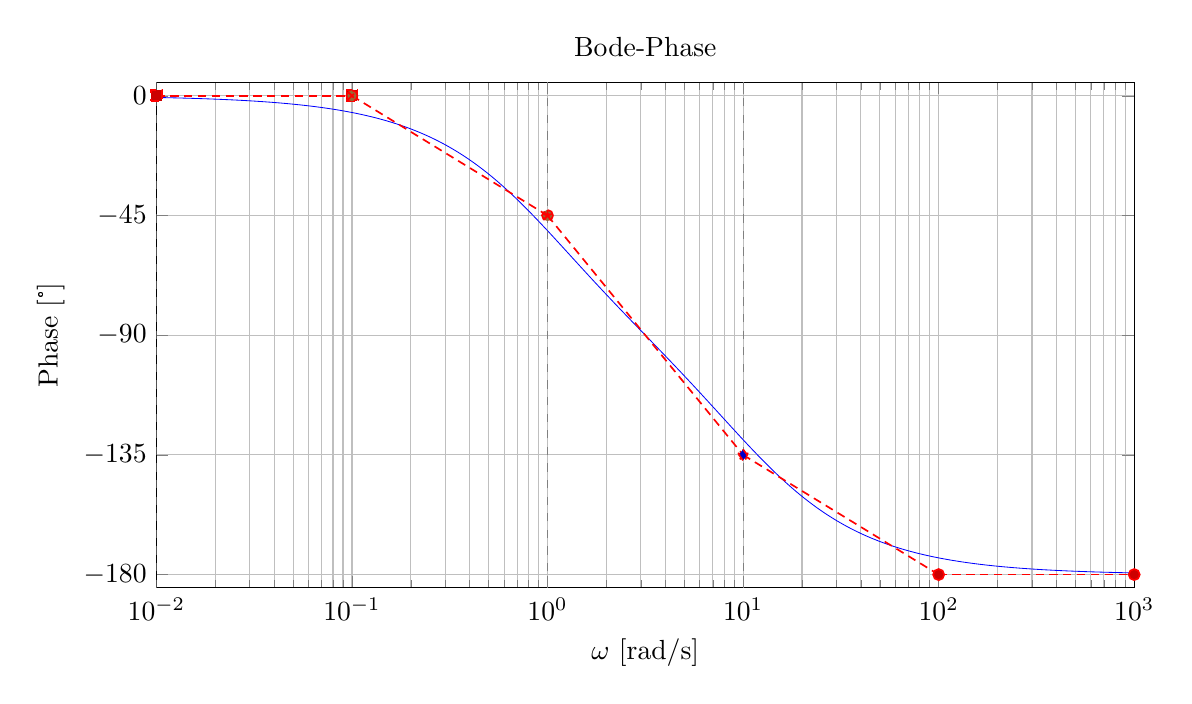
\begin{tikzpicture}
\begin{semilogxaxis}[
  width=14cm,height=8cm,
  xmin=1e-2,xmax=1e3,
  ymin=-185,ymax=5,
  xlabel={$\omega$ [rad/s]},
  ylabel={Phase [°]},
  ytick distance=45,
  grid=both,
  title={Bode-Phase}
]
\addplot[
  domain=1e-2:1e3,
  samples=600,
  mark=none,
  line width=0.3pt,
  blue
] {-atan(x) - atan(x/10)};
\addplot+[domain=1e-2:1e-1,samples=2,dashed,dash pattern=on 3pt off 2pt,line width=0.6pt,red] {0};
\addplot+[domain=1e-1:1e0,samples=2,dashed,dash pattern=on 3pt off 2pt,line width=0.6pt,red] {-45 - 45*ln(x)/ln(10)};
\addplot+[domain=1e0:1e1,samples=2,dashed,dash pattern=on 3pt off 2pt,line width=0.6pt,red]{-45 - 90*ln(x)/ln(10)};
\addplot+[domain=1e1:1e2,samples=2,dashed,dash pattern=on 3pt off 2pt,line width=0.6pt,red] {-135 - 45*ln(x/10)/ln(10)};
\addplot+[domain=1e2:1e3,samples=2,dashed,dash pattern=on 3pt off 2pt,line width=0.6pt,red] {-180};
\draw[gray,dashed] (rel axis cs:0,0) -- (rel axis cs:0,1);
\draw[gray,dashed] (axis cs:1,\pgfkeysvalueof{/pgfplots/ymin}) -- (axis cs:1,\pgfkeysvalueof{/pgfplots/ymax});
\draw[gray,dashed] (axis cs:10,\pgfkeysvalueof{/pgfplots/ymin}) -- (axis cs:10,\pgfkeysvalueof{/pgfplots/ymax});
\node[gray,anchor=south east] at (axis cs:1,\pgfkeysvalueof{/pgfplots/ymax}) {\scriptsize Nullstelle $\omega_z=1$ (RHP)};
\node[gray,anchor=south east] at (axis cs:10,\pgfkeysvalueof{/pgfplots/ymax}) {\scriptsize Pol $\omega_p=10$};
\end{semilogxaxis}
\end{tikzpicture}
\end{center}
\newpage
\subsection{Erklärung}
\vspace{5mm}
\begin{description}[leftmargin=1.2em,labelsep=.6em,font=\bfseries]
\item[Schritt 1] DC-Faktor $1$: $H(0)=1\Rightarrow |H|_{\mathrm{DC}}=0\,\mathrm{dB}$ ohne Anfangssteigung; Phase $\approx0^\circ$.
\item[Schritt 2] Nullstelle bei $\omega_z=1\,\mathrm{rad/s}$ in der rechten Halbebene: Magnitude-Beitrag identisch zur LHP-Nullstelle $\Rightarrow$ ab $\omega=1$ Anstieg um $+20\,\mathrm{dB/dec}$. Phasenbeitrag ist nicht-minimumphasig: Übergang $0^\circ\to-90^\circ$ über $\omega\in[0.1,10]$; Geradennäherung $-45^\circ-45\log_{10}\omega$ liefert $\angle H(\j1)\approx-45^\circ$. Exakt liegt die Magnitude bei $\omega=1$ bei $20+10\log_{10}2-10\log_{10}101\approx+2.96\,\mathrm{dB}$.
\item[Schritt 3] Pol bei $\omega_p=10\,\mathrm{rad/s}$: ab $\omega=10$ Steigungswechsel um $-20\,\mathrm{dB/dec}$; für $\omega\gg10$ ergibt sich konstanter Betrag $\approx+20\,\mathrm{dB}$. Phasenabfall des Pols um weitere $90^\circ$ über $\omega\in[1,100]$; Geradennäherung $-45^\circ-45\log_{10}(\omega/10)$. Zusammengesetzt: Phase $\approx0^\circ$ für $\omega\ll0.1$, $\approx-90^\circ$ um $\omega\approx10$, und $\approx-180^\circ$ für $\omega\gg100$.
\end{description}

\vspace{0.5cm}
\medskip
\noindent\textbf{Stückweise Näherung}
\[
|H(\j\omega)|_{\mathrm{dB}}\approx
\begin{cases}
0,& \omega\ll1,\\[4pt]
20\log_{10}\omega,& 1\ll\omega\ll10,\\[4pt]
20,& \omega\gg10,
\end{cases}
\qquad
\]
\newpage